\documentclass[11pt,ngerman]{article}
\usepackage{geometry}
\usepackage[T1]{fontenc}
\usepackage[utf8]{inputenc}
\usepackage{babel}
\usepackage{hyperref}
\usepackage{lmodern}%get scalable font
\usepackage{titling}
\usepackage{relsize}
\usepackage{biblatex}
\usepackage{glossaries}
\usepackage{paralist}
\usepackage[table, dvipsnames]{xcolor}
\usepackage{booktabs}
\usepackage{tabularx}
\usepackage{float}
\restylefloat{table}
\usepackage{setspace}
\usepackage{multicol}
\usepackage{graphicx}
\usepackage[space]{grffile}
\usepackage[most]{tcolorbox}
\usepackage{enumitem}
\usepackage{textcomp}

% Link colors
\hypersetup{
    colorlinks,
    linkcolor={blue},
    citecolor={red},
    urlcolor={blue}
}

\geometry{a4paper, top=25mm, left=25mm, right=25mm, bottom=20mm,
    headsep=10mm, footskip=12mm}

% Glossary
% Das Glossar definiert alle wichtigen Begriffe zur Sicherstellung einer einheitlichen Terminologie.
% Es sollen keine allgemeinen Begriffe erklärt werden, die den Adressaten bekannt sind (z. B. Java, CPU etc.).
% Glossareinträge müssen im Text verwendet werden, damit diese im Glossar im Appendix \printglossary angezeigt werden
\makeglossaries
\loadglsentries{glossary} % loads glossary definitions from external file

\pretitle{\begin{center}\linespread{1.5}\huge}
    \posttitle{\par\end{center}\vspace{0.5em}}

% double quotes macro
% usage: \quotes{arg1}  => in text: "arg1"
\newcommand{\quotes}[1]{``#1''}

\begin{document}

    \title{Tron Licht-Motorräder Computerspiel\\
        \vspace{1cm}
        Lösungsarchitektur \\
        \vspace{0.5cm}
        \small{}ZHAW  School of Engineering
        \vspace{1.5cm}
    }
    \author{
        Akca, Deniz\\
        \small{akcaden1@students.zhaw.ch}
        \and
        Holenstein, Christian\\
        \small{holenchr@students.zhaw.ch}
        \and
        Huber, Patrick\\
        \small{huberpa4@students.zhaw.ch}
        \and
        Iten, Mike\\
        \small{itenmik1@students.zhaw.ch}
        \vspace{1.5cm}
    }
   \date{\today}

    \maketitle
    \newpage

    \tableofcontents
    \listoftables
    \listoffigures
    \newpage

    % First section
    \section{Anwendungsfälle}
        Anwendungsfälle Übersicht:
        \begin{multicols}{2}
            \begin{itemize}
               \item  \hyperref[ssec:UC1Lobbyerstellen]{UC1: Lobby erstellen - \quotes{fully dressed}}
                \item\hyperref[ssec:UC2Spielspielen]{UC2: Spiel spielen - \quotes{fully dressed}}
                \item \hyperref[sssec:UC3EinAusloggen]{UC3: Ein \& Ausloggen  - \quotes{casual}}
                \item \hyperref[sssec:UC4Lobbybeitreten]{UC4: Lobby beitreten - \quotes{casual}}
                \item \hyperref[sssec:UC5Registrieren]{UC5: Registrieren - \quotes{brief}}
                \item \hyperref[sssec:UC6Passwortsetzen]{UC6: Passwort zurücksetzen - \quotes{brief}}
                \item  \hyperref[sssec:UC7Freundeeinladen]{UC7: Freunde einladen - \quotes{brief}}
                \item \hyperref[sssec:UC8Statistikenbetrachten]{UC8: Statistiken betrachten - \quotes{brief}}
           \end{itemize}
        \end{multicols}

        \subsection{Anwendungsfalldiagramm}
            \begin{figure}[H]
                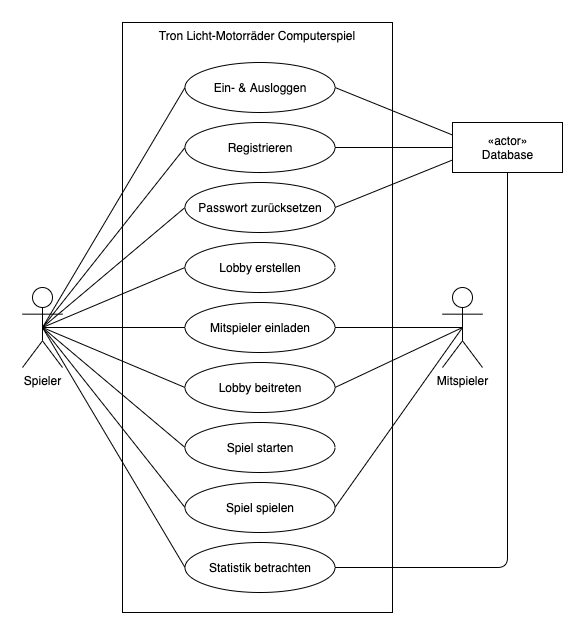
\includegraphics[scale=0.77]{figures/Use-case-modell.png}
                \caption{Anwendungsfalldiagramm - Tron Licht-Motorräder Computerspiel}
            \end{figure}

        \subsection{Hauptanwendungsfälle}
            Wir haben zwei Hauptanwendungsfälle identifiziert:
             \begin{itemize}
                \item  \hyperref[ssec:UC1Lobbyerstellen]{UC1: Lobby erstellen - \quotes{fully dressed}}
                \item\hyperref[ssec:UC2Spielspielen]{UC2: Spiel spielen - \quotes{fully dressed}}
            \end{itemize}
            Die Hauptanwendungsfälle werden in den nächsten zwei Abschnitten detailliert ausgeführt.

            \subsubsection{UC1: Lobby erstellen - \quotes{fully dressed}}
            \label{ssec:UC1Lobbyerstellen}
                \begin{tcolorbox}[enhanced, breakable, sharp corners, width=\dimexpr\textwidth-15mm\relax ,enlarge left by=10mm ,fontupper=\linespread{1.1}\selectfont, boxrule=1pt, title={UC1: Lobby erstellen}, colback=white, colframe=gray!22, coltitle=black]

                    \textbf{Anwendungsfall:} Lobby erstellen \\
                    \textbf{Ebene:} Anwenderziel \\
                    \textbf{Primärakteur:} Spieler \\
                    \textbf{Stakeholder und Interessen:}
                    \begin{itemize}
                        \item \textit{Spieler}: Möchte mit anderen Spielern zusammen in einer \Gls{Lobby} beitreten oder seine eigene \Gls{Lobby} erstellen. Kann die Rolle des Lobby-Erstellers haben.
                        \item \textit{Mitspieler}: Möchten mit anderen Spielern zusammen in einer \Gls{Lobby} beitreten. Kann die Rolle des Lobby-Erstellers haben.
                        \item \textit{Lobby-Ersteller}:  Möchte das Spiel starten, wenn alle Spieler bereit sind.
                        \item \textit{System}: Möchte mehrere Spieler in einer \Gls{Lobby} haben, um ein Spiel starten zu können.
                    \end{itemize}
                    \textbf{Vorbedingungen:} Alle Spieler sind entweder mit einem persönlichen oder Gastkonto angemeldet.\\
                    \textbf{Nachbedingungen:} Mehrere Spieler oder auch einzelne Spieler befinden sich in \Glspl{Lobby}. Das System ist in der Lage in den \Glspl{Lobby} mit mehreren Spielern ein Spielgang zu starten. \\
                    \\  \textbf{Standardablauf:}
                    \begin{enumerate}
                        \item Spieler/Mitspieler wechselt zur Lobbyansicht der Anwendung.
                        \item Spieler/Mitspieler wählt eine bestehende öffentliche \Gls{Lobby} aus.
                        \item Spieler/Mitspieler tritt diese \Gls{Lobby} bei.
                        \item Spieler und Mitspieler warten in \Gls{Lobby} auf weitere Mitspieler..
                        \item Spieler/Mitspieler klicken auf \quotes{Bereit}
                        \item Lobby-Ersteller startet das Spiel.
                        \item System überprüft ob alle Spieler in der \Gls{Lobby} bereit sind.
                    \end{enumerate}
                    \textit{Falls nicht alle Spieler bereit sind, muss der Lobby-Ersteller zu einem weiteren Zeitpunkt nochmals Schritt 6 ausführen. Erst wenn alle Spieler bereit sind, wird mit Schritt 8 fortgefahren.}
                    \begin{enumerate}[resume]
                        \item System startet das Spiel.
                    \end{enumerate}
                    \textit{Es ist nun nicht mehr möglich - als Spieler oder Mitspieler - dieser \Gls{Lobby} beizutreten.} \\
                    \textit{Spiel wird gespielt …, Ende des Spiels.}
                    \begin{enumerate}[resume]
                        \item System öffnet \Gls{Lobby} wieder
                    \end{enumerate}
                    \textit{Spieler/Mitspieler können \Gls{Lobby} beitreten. Punkt 3 bis 9 wiederholen sich, bis Spieler sich entscheidet, das Spiel oder die \Gls{Lobby} zu verlassen.} \\
                    \\ \textbf{Erweiterungen (oder alternative Abläufe):}
                    \begin{itemize}
                        \item[2a.] Spieler können eigene \Gls{Lobby} erstellen:
                        \begin{enumerate}
                            \item Spieler klickt auf \Gls{Lobby} erstellen.
                            \item Spieler wählt ob die \Gls{Lobby} öffentlich zugänglich (public) ist oder nur für Freunde (private).
                            \item System erstellt eine \Gls{Lobby}.
                            \item System fügt den Spieler als Lobby-Ersteller der \Gls{Lobby} hinzu.
                        \end{enumerate}
                        \item[2b.] Spieler können privaten \Glspl{Lobby} von Freunden über einen Link beitreten:
                        \begin{enumerate}
                            \item Spieler öffnet Einladung.
                            \item Spieler öffnet den Link im Browser.
                            \item System fügt Spieler der \Gls{Lobby} des Freundes hinzu.
                        \end{enumerate}
                        \item[4a.] Spieler können \Gls{Lobby} verlassen:
                        \begin{enumerate}
                            \item Spieler/Mitspieler verlassen \Gls{Lobby}
                        \end{enumerate}
                        \item[4b.] Spieler/Mitspieler können weiter in der \Gls{Lobby} bleiben und weiterspielen:
                        \begin{enumerate}
                            \item Spieler/Mitspieler verlassen die \Gls{Lobby} nicht
                        \end{enumerate}
                    \end{itemize}
                    \textbf{Spezielle Anforderungen:}
                    \begin{itemize}
                        \item Sobald ein Mitspieler der \Gls{Lobby} beigetreten ist, läuft ein Timer. Falls der Timer abgelaufen ist und der Mitspieler noch nicht bestätigt hat, wird dieser automatisch abgelehnt.
                        \item Maximale Spieleranzahl muss eingehalten werden. Es gibt eine obere Grenze von Mitspielern, die durch den Spieler definiert wird.
                        \item Internationalisierung der Sprache in den Textanzeigen.
                    \end{itemize}

                \end{tcolorbox}

            \subsubsection{UC2: Spiel spielen - \quotes{fully dressed}}
            \label{ssec:UC2Spielspielen}
                \begin{tcolorbox}[enhanced, breakable, sharp corners, width=\dimexpr\textwidth-15mm\relax ,enlarge left by=10mm ,fontupper=\linespread{1.1}\selectfont, boxrule=1pt, title={UC2: Spiel spielen}, colback=white, colframe=gray!22, coltitle=black]

                    \textbf{Anwendungsfall:} Spiel spielen \\
                    \textbf{Ebene:} Anwenderziel \\
                    \textbf{Primärakteur:} Spieler \\
                    \textbf{Stakeholder und Interessen:}
                    \begin{itemize}
                        \item \textit{Spieler}: Möchte als letzter Spieler übrig bleiben
                        \item \textit{Mitspieler}: Möchte als letzter Spieler übrig bleiben.
                        \item \textit{Lobby-Ersteller}:  Möchte das Spiel starten, wenn alle Spieler bereit sind.
                        \item \textit{System}: Möchte alle Spieler - bereit zum spielen - in einer \Gls{Lobby} haben, um ein Spiel starten zu können.
                    \end{itemize}
                    \textbf{Vorbedingungen:} Mindestens 2 Spieler sind im Spiel.\\
                    \textbf{Nachbedingungen:} Der letzte Spieler im Spiel wurde Sieger. Spiel wurde erfolgreich beendet. \Gls{Lobby} wird erneut angezeigt. \\
                   \\  \textbf{Standardablauf:}
                    \begin{enumerate}
                        \item System lädt Spiel.
                        \item System platziert Spieler/Mitspieler (Spielcharakter) in einem gewissen Abstand zum Spielfeldrand und zu den Mitspielern, jeweils in möglichst entgegengesetzter Richtung, auf dem Spielfeld.
                        \item System zeigt Countdown an. Nach Ablauf des Countdowns beginnt das Spiel.
                        \item System beginnt Startbewegung der Spieler mit konstanter Geschwindigkeit in Richtung Spielfeldmitte.
                    \end{enumerate}
                    \textit{Alle Spieler/Mitspieler auf dem Spielfeld behalten die konstante Geschwindigkeit bei bis zum Ausscheiden oder Ende des Spiels.}
                    \begin{enumerate}[resume]
                        \item System erzeugt Hindernis vom Startpunkt des Spielers/Mitspielers bis zu dessen aktueller Position.
                        \item System übergibt Spieler/Mitspieler die Kontrolle des jeweiligen Spielcharakters.
                    \end{enumerate}
                    \textit{Schritt 4 - 6 folgen ohne Zeitverzögerung aufeinander.}
                    \begin{enumerate}[resume]
                        \item Spieler/Mitspieler können, durch drücken einer Pfeiltaste, die Richtung um jeweils exakt 90\textdegree\ ändern.
                        \item Das durch den Spieler/Mitspieler erzeugte Hindernis, wächst mit der Bewegung und in der jeweiligen Bewegungsrichtung.
                    \end{enumerate}
                    \textit{Das vom Spieler/Mitspieler erzeugte Hindernis, bleibt auf dem Spielfeld bestehen bis zum Ausscheiden oder Sieg des Spielers/Mitspielers, in allen folgenden Schritten.}
                    \begin{enumerate}[resume]
                        \item System koordiniert in kurzen Intervallen alle Bewegungen der Spieler/Mitspieler und überprüft deren Positionen und etwaige Kollisionen.
                    \end{enumerate}
                    \textit{System wiederholt Schritt 7 - 9 bis Kollision erkannt wird.}
                    \begin{enumerate}[resume]
                        \item System entfernt Spieler/Mitspieler mit Kollision vom Spielfeld und zeigt eine entsprechende Meldung an.
                    \end{enumerate}
                    \textit{System wiederholt Schritt 7 - 10 bis ein einziger Spieler/Mitspieler auf dem Spielfeld übrig bleibt.}
                    \begin{enumerate}[resume]
                        \item System zeigt bei letztem Spieler/Mitspieler eine Siegesmeldung an.
                        \item System beendet das Spiel.
                        \item System zeigt die Statistiken des Spiels bei allen Spielern/Mitspielern an.
                        \item System öffnet - nach Ablauf eines Timers  - erneut die \Gls{Lobby}.
                    \end{enumerate}
                    \textbf{Erweiterungen (oder alternative Abläufe):}
                    \begin{itemize}
                        \item[?a.] blah
                            \begin{enumerate}
                                \item blah
                                \item blah
                                \item blah
                            \end{enumerate}
                    \end{itemize}
                    \textbf{Spezielle Anforderungen:}
                     \begin{itemize}
                        \item blah
                    \end{itemize}

                \end{tcolorbox}

            \newpage
            \subsubsection{System-Sequenzdiagramm (SSD)}
                 Das System-Sequenzdiagramm für \quotes{Lobby erstellen} und \quotes{Spiel spielen}:
                 \begin{figure}[H]
                     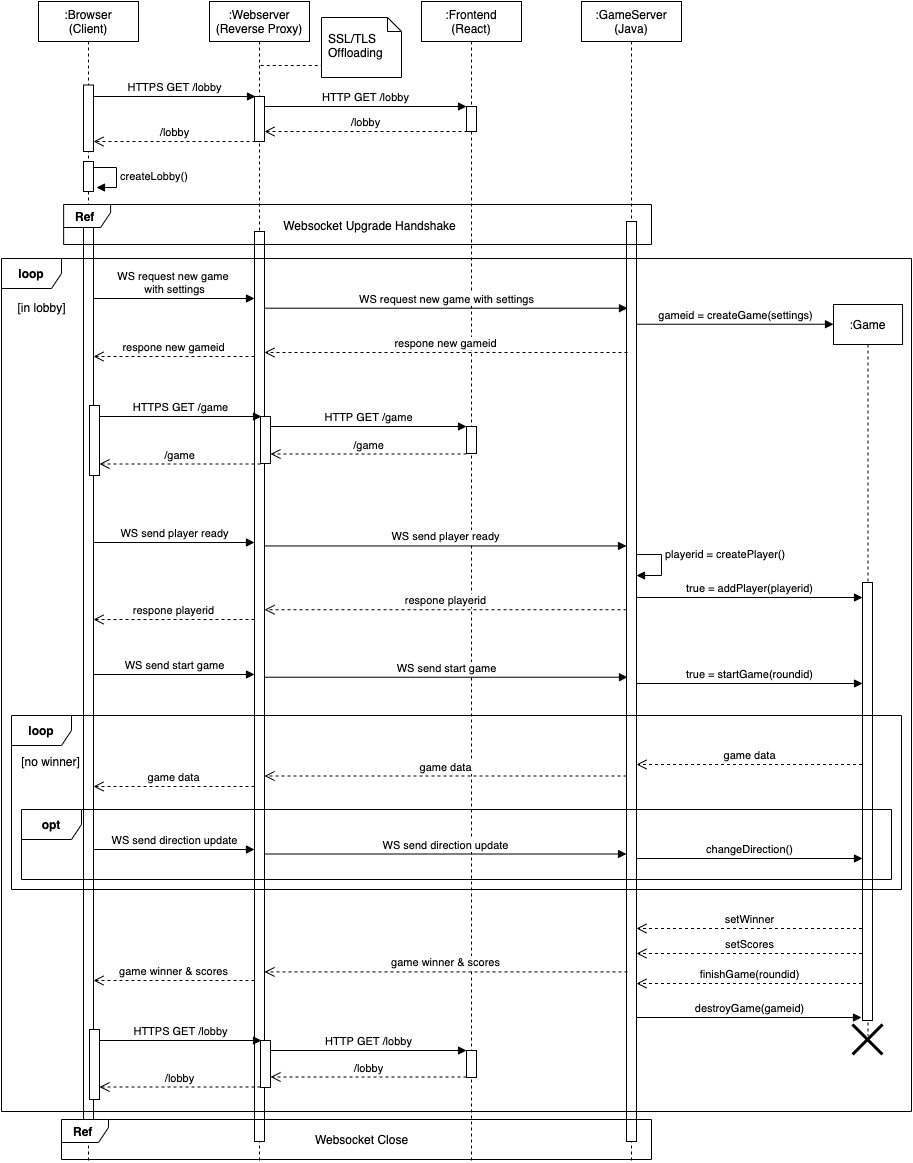
\includegraphics[scale=0.5]{figures/SystemSequenceDiagram.png}
                     \caption{System-Sequenzdiagramm - \quotes{Lobby erstellen} \&  \quotes{Spiel spielen}}
                 \end{figure}
                 \newpage
                \noindent \textbf{Referenz: \Gls{Websocket} Upgrade Handshake} \\
                \autoref{fig:SSDReferenzWebsocketUpgrade} zeigt den Upgrade Request der HTTP(S) Verbindung  zu \Gls{Websocket}.
                \begin{figure}[H]
                    \centering
                    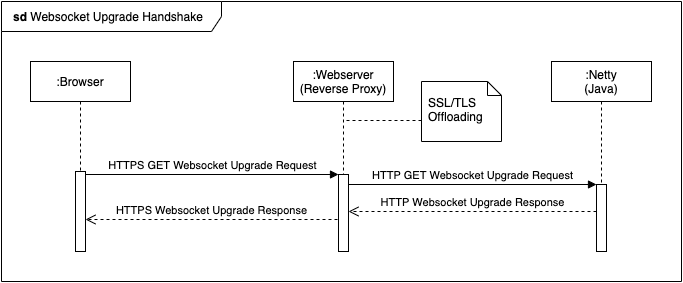
\includegraphics[scale=0.6]{figures/SSD-Websocket_Upgrade_Handshake.png}
                    \caption{SSD Referenz - \Gls{Websocket} Upgrade Handshake}
                    \label{fig:SSDReferenzWebsocketUpgrade}
                \end{figure}
                \noindent \textbf{Referenz: \Gls{Websocket} Close} \\
                \autoref{fig:SSDReferenzWebsocketClose} zeigt das schliessen der \Gls{Websocket}-Verbindung.
                \begin{figure}[H]
                    \centering
                    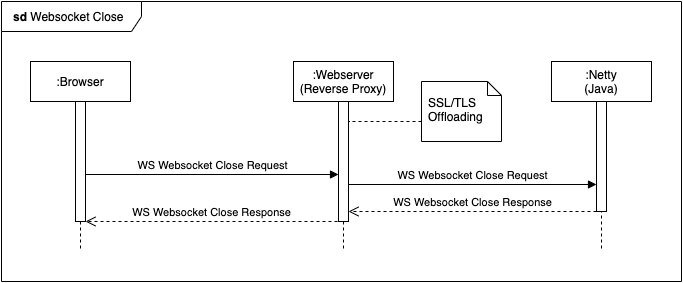
\includegraphics[scale=0.6]{figures/SSD-Websocket_Close.png}
                    \caption{SSD Referenz - \Gls{Websocket} Close}
                    \label{fig:SSDReferenzWebsocketClose}
                \end{figure}

        \subsection{Übrige Anwendungsfälle}
        \subsubsection{UC3: Ein \& Ausloggen  - \quotes{casual}}
        \label{sssec:UC3EinAusloggen}
        \begin{tcolorbox}[enhanced, breakable, sharp corners, width=\dimexpr\textwidth-15mm\relax ,enlarge left by=10mm ,fontupper=\linespread{1.1}\selectfont, boxrule=1pt, title={UC3: Ein \& Ausloggen }, colback=white, colframe=gray!22, coltitle=black]
        	\textit{Standardszenario:} Der Spieler navigiert sich zum Login-Bereich der Anwendung. Im Login-Bereich gibt er die korrekten Eingabedaten seines Kontos ein. Die Anwendung überprüft die Eingabedaten und meldet den Spieler an. Der
        	Spieler ist nun in der Anwendung mit seinem persönlichen Konto angemeldet.\newline
        	\newline
        	\textit{Alternative Szenarios:} \newline
        	Der Spieler gibt die falschen Eingabedaten für ein Konto ein. Das System weist den Spieler
        	daraufhin, dass die Eingabedaten falsch sind und schlägt dem Spieler vor noch einmal die  Eingabedaten einzugeben. \newline
        	\newline
        	Der Spieler möchte sich aus dem System ausloggen. Der Spieler navigiert sich in der Anwendung oben rechts und wählt die Funktion «Logout» aus. Das System beendet die Session und der Spieler wird als Gast neu angemeldet.
        \end{tcolorbox}

        \subsubsection{UC4: Lobby beitreten - \quotes{casual}}
        \label{sssec:UC4Lobbybeitreten}
        \begin{tcolorbox}[enhanced, breakable, sharp corners, width=\dimexpr\textwidth-15mm\relax ,enlarge left by=10mm ,fontupper=\linespread{1.1}\selectfont, boxrule=1pt, title={UC4: Lobby beitreten }, colback=white, colframe=gray!22, coltitle=black]
        	\textit{Standardszenario:} Der Spieler navigiert auf der Startseite zu dem Lobbybereich, dort kann er einer öffentlichen Lobby beitreten. \newline
        	Nun befindet sich der Spieler in einer Lobby mit weiteren Mitspielern.\newline
        	\newline
        	\textit{Alternative Szenarios:} \newline
        	Der Spieler erhält einen Link eines Freundes. Mit dem Link kann der Spieler einer privaten Lobby beitreten. \newline
        	Er befindet sich nun in derselben Lobby mit seinem Freund.
        \end{tcolorbox}

        \subsubsection{UC5: Registrieren - \quotes{brief}}
        \label{sssec:UC5Registrieren}
        \begin{tcolorbox}[enhanced, breakable, sharp corners, width=\dimexpr\textwidth-15mm\relax ,enlarge left by=10mm ,fontupper=\linespread{1.1}\selectfont, boxrule=1pt, title={UC5: Registrieren}, colback=white, colframe=gray!22, coltitle=black]
        	Der Spieler navigiert sich zum Registrier-Bereich der Anwendung. Im Registrier-Bereich gibt er seinen Usernamen, Passwort und E-Mail an.\newline
        	Die Anwendung überprüft ob der Username bereits belegt ist. Der Spieler besitzt nun ein eigenes Konto
        \end{tcolorbox}

        \subsubsection{UC6: Passwort zurücksetzen - \quotes{brief}}
        \label{sssec:UC6Passwortsetzen}
        \begin{tcolorbox}[enhanced, breakable, sharp corners, width=\dimexpr\textwidth-15mm\relax ,enlarge left by=10mm ,fontupper=\linespread{1.1}\selectfont, boxrule=1pt, title={UC6: Passwort zurücksetzen}, colback=white, colframe=gray!22, coltitle=black]
        	Der Spieler navigiert sich zum Login-Bereich der Anwendung. Dort hat er die Möglichkeit sein Passwort zurück zu setzen.\newline
        	Nun kann der Spieler ein neues Passwort angeben.
        \end{tcolorbox}

        \subsubsection{UC7: Freunde einladen - \quotes{brief}}
        \label{sssec:UC7Freundeeinladen}
        \begin{tcolorbox}[enhanced, breakable, sharp corners, width=\dimexpr\textwidth-15mm\relax ,enlarge left by=10mm ,fontupper=\linespread{1.1}\selectfont, boxrule=1pt, title={UC7: Freunde einladen}, colback=white, colframe=gray!22, coltitle=black]
        	Der Spieler erstellt eine private Lobby. Er erhält einen Link, mit welchem Freunde beitreten können.\newline
        	Sobald seine Freunde den Link benutzen, befinden sie sich nun mit dem Spieler in derselben Lobby.
        \end{tcolorbox}

        \subsubsection{UC8: Statistiken betrachten - \quotes{brief}}
        \label{sssec:UC8Statistikenbetrachten}
        \begin{tcolorbox}[enhanced, breakable, sharp corners, width=\dimexpr\textwidth-15mm\relax ,enlarge left by=10mm ,fontupper=\linespread{1.1}\selectfont, boxrule=1pt, title={UC8: Statistiken betrachten}, colback=white, colframe=gray!22, coltitle=black]
        	Der Spieler navigiert auf der Startseite der Anwendung zu den Statistiken. Dort ist eine Liste einsehbar, in welcher die besten Spieler mit ihren Punkten aufgelistet sind.
        \end{tcolorbox}

    \section{Zusätzliche Anforderungen}
    	Es ist wichtig, konkrete Anforderungen für unser Spiel zu definieren, damit die Erwartungen der Spieler erfüllt werden können. Hierbei soll uns das FURPS+ Modell weiter helfen. Im Folgenden werden die einzelnen Punkte genauer definiert.
        \subsection{Funktionalität}
        Um das Spiel so einfach wie möglich zu gestalten, haben wir uns dazu entschieden, dass bei dem Erstbetreten des Spiels ein Gastaccount zugewiesen wird. Dadurch müssen Spieler, welche nur für ein kurzes Spielvergnügen vorbei schauen, keine zusätzliche Angaben machen oder sonstige Zeit verlieren. Der normale Registrierungs- oder Loginvorgang kann zu jederzeit benutzt werden. Dies gibt uns danach die Möglichkeit auf benutzerspezifische Erweiterungen wie zum Beispiel In-App Käufe oder mögliche, bevorzugte Farben für das Licht-Motorrad im Spiel. Die Spieler, die nur mit einem Gastaccount angemeldet sind, haben demnach weniger Möglichkeiten. Der Gast wird auch nicht in der Punktestatistik aufgeführt.\newline
        \newline
        % TODO \autoref verwenden für Verweiss auf andere Section
        Damit die Spieler zusammen einer Lobby beitreten können, benutzen wir eine Server-Client-Architektur, welche ausführlicher in der Software Architektur ersichtlich ist. Spezielle Sicherheitsmassnahmen nicht notwendig, da keine sensiblen Daten übertragen werden. Standard-Sicherheitsmassnahmen, wie verschlüsselte Datenübertragung über HTTPS, sind gewährleistet.
        \subsection{Benutzbarkeit}
        Eines der wichtigsten Aspekte für uns, ist die Benutzbarkeit. Das Spiel soll übersichtlich, intuitiv und einfach gestaltet sein. Der Spieler muss mit wenigen Klicks alle wichtigen Funktionalitäten erreichen können. Damit wir dies anbieten können, benutzen wir ein rudimentäres Design und eine \Gls{SPA}-Applikation, welche diesen Aspekt unterstützt. Zusätzlich wird - zum Beispiel - der \Gls{Lobby} beitreten Button direkt auf der ersten Seite ersichtlich sein, welche der Spieler nach dem betreten der Applikation sieht.
        \begin{figure}[H]
            \centering
            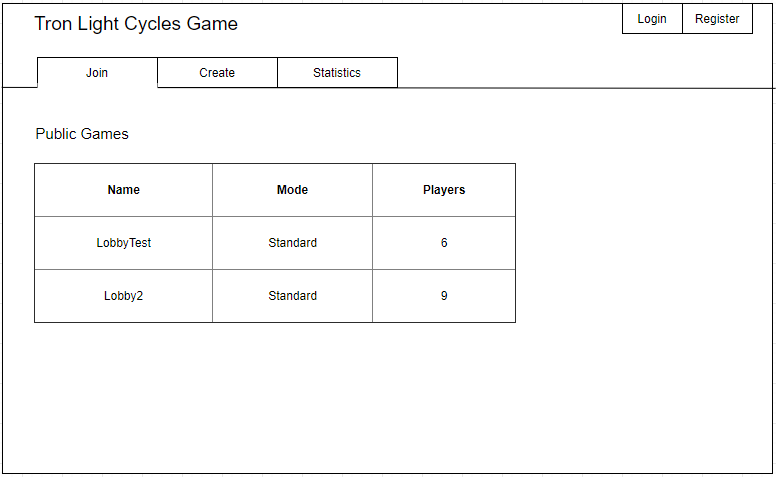
\includegraphics[scale=0.6]{figures/Mockup_Join.png}
            \caption{Mockup Join}
            \label{fig:MockupJoin}
        \end{figure}
        \subsection{Zuverlässigkeit}
        Wir können mit Sicherheit sagen, dass unsere Applikation nicht sonderlich anfällig für Ausfälle ist. Da das Spiel nur eine geringe Leistung beansprucht, verringert das die Fehlerquellen enorm. Die Applikation ist auch Clientabhängig. Das bedeutet, falls ein Spieler Verbindungsprobleme hat oder andere Schwierigkeiten, dann kann er verlieren. Die Lobby liegt auf dem Server, somit ist gewährleistet, dass falls der Spieler, welche die Lobby erstellt hat, Verbindungsprobleme hat, das Spiel weiterhin normal abläuft. Dies ist ebenso ein wichtiger Aspekt für uns, damit das Spiel reibungslos ohne Unterbrüche ablaufen kann.
        \subsection{Effizienz}
    	Da wie bereits erwähnt das Spiel nur eine geringe Leistung beansprucht, ist die Effizienz gut und zuverlässig. Hier spielt leider auch wieder der Client eine Rolle. Da der Server und der Client in Verbindung stehen und der Client Verbindungsprobleme oder sonstige Verzögerungen hat, kommt es schnell zu kurzen Unterbrechungen für den Spieler. Dies ist kaum zu vermeiden.
        \subsection{Änderbarkeit (Wartbarkeit)}
    	Die Applikation ist nur über den Browser erreichbar, dies macht die Wartbarkeit um einiges einfacher. Die diversen Browser müssen natürlich getestet werden und kompatibel sein. Die wichtigsten Browser sind Firefox, Google Chrome und Internet Explorer.  Das Testen neuerer Versionen der einzelnen Browser schliesst dies mit ein, um die Zuverlässigkeit weiterhin anbieten zu können.
        \subsection{Internationalisierung}
        In der ersten lauffähigen Version wird Englisch verwendet. Später sollen andere Sprachen folgen um grössere Reichweite zu generieren.
        \subsection{Einschränkungen}

        \subsubsection{Designeinschränkungen}
        Wir benutzen React und Material UI für das Design, da Material UI bereits einige Bibliotheken, beziehungsweise vordefinierte  Bausteine zur Verfügung stellt. Da wir mit einer \Gls{SPA} arbeiten wird Routing vorerst nicht nötig sein.
        \subsubsection{Implementierungseinschränkungen}
    	Um die Applikation so wartbar wie möglich zu behalten, wird alles so gut wie möglich mit Clean Code implementiert. Dies wird auch im späteren Verlauf des Implementierungsvorgangs immer wieder überprüft. Bei Git benutzen wir das \Gls{Continuous Integration} (CI), dies ermöglicht es uns nur kompilierbaren Code hinzuzufügen um einige Fehlerquellen bereits auszuschliessen.
        \subsubsection{Schnittstelleneinschränkungen}

    \section{Domänenmodell}
    \begin{figure}[H]
        \centering
        \makebox[\textwidth][c]{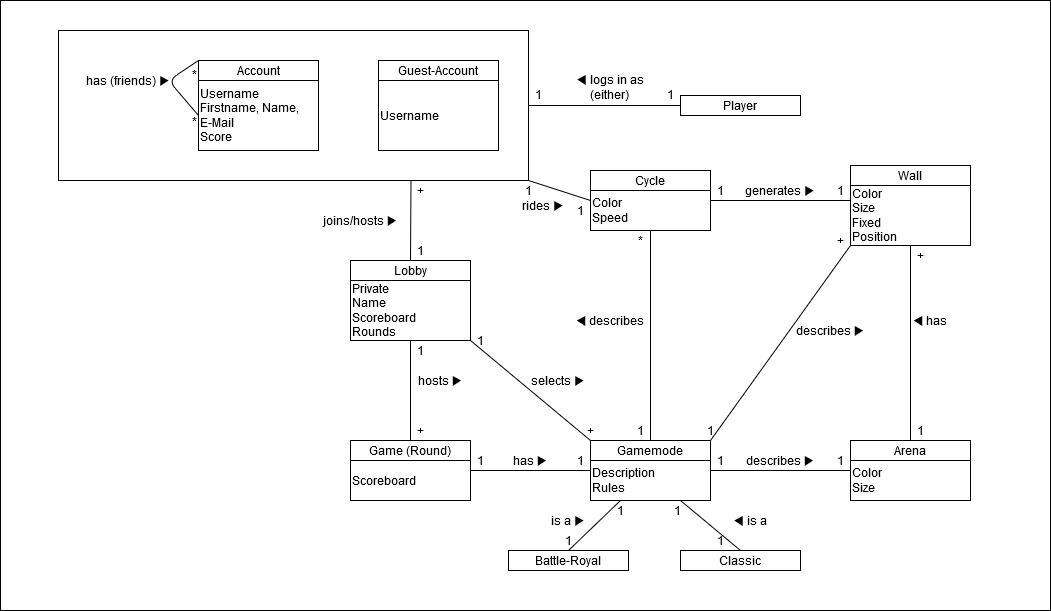
\includegraphics[width=1.1\textwidth]{figures/domain_model.png}}
        \caption{Domänenmodell - Tron Licht-Motorräder Computerspiel}
        \label{fig:DomainModel_TronLightCycles}
    \end{figure}
	\subsection{Login und Gast-Account}
		Der Spieler hat die Freiheit sich mit einem anonymen Gastkonto  oder mit einem registriertem Konto anzumelden. Der Spieler kann sich in der Applikation nicht mit beiden Kontoarten gleichzeitig identifizieren.

	\subsection{Spielemodi}
		Ein Spielmodus beeinflusst das Spiel, zwei Spielmodi werden schon implementiert sein. Im Spielmodus sind Eigenschaften der Licht-Motorräder und die Grösse der Arena definiert, so auch Spielablauf.


    \section{Softwarearchitektur}
        Das System wurde in vier Hauptkomponenten aufgeteilt. Dies erlaubt eine zielgerichtete Auswahl der verwendeten Programmiersprachen und Nutzung von Frameworks. Die Hauptkomponenten - jeweils dem Frontend oder Backend zugeordnet - sind:
        \begin{multicols}{2}
            \begin{itemize}
                \item \textbf{Frontend}
                \begin{itemize}
                    \item Website
                    \item Spieleclient
                \end{itemize}
                \item \textbf{Backend}
                \begin{itemize}
                    \item Spieleserver
                    \item Datenbank
                \end{itemize}
            \end{itemize}
        \end{multicols}

        \noindent Aufgrund des Vorwissens des Projektteams, standen grundsätzlich zwei Sprachen für die Implementation des Systems zur Auswahl: Java und Javascript. Im folgenden werden die oben beschriebenen Hauptkomponenten genauer beschrieben und die jeweilige Wahl der Sprache und der Frameworks erläutert.

        \subsection{Website}
        Die Website wird in Javascript mit dem Framework \Gls{React} realisiert. \Gls{React} erlaubt es, die Webseite als moderne \Gls{SPA}-Applikation zu erstellen. Eine \Gls{SPA} trägt durch ihr dynamisches Laden von Inhalten, massgeblich zur freundlichen und intuitiven Benutzung der Webseite bei. Dies wäre beispielsweise mit einer \Gls{JSP}-Implementation nicht möglich. \Gls{React} nutzt wiederverwendbare  \quotes{Bausteine}, sogenannte \quotes{Komponenten}. Die Komponenten erlauben ein modularer Aufbau des gesamten Frontends.

        \subsection{Spieleclient}
        Der Spieleclient  kommuniziert direkt mit dem Spieleserver über eine \Gls{Websocket}-Verbindung. Momentan ist der Spieleclient  in zwei \Gls{React}-Komponenten aufgeteilt. Die eine Komponente kümmert sich um die Animation und die zweite, einfachere um die Darstellung mithilfe des \Gls{HTML5 Canvas} Elements.

        \label{SoftwarearchitekturGameServer}
        \subsection{Spieleserver \Gls{Game Server}}
        Der \Gls{Game Server} setzt sich grundsätzlich aus zwei Teilen zusammen. Zum einen aus der Geschäftslogikschicht, also dem Teil, der jeweils ein Spiel generiert und laufend den aktuellen Spielzustand berechnet. Zum anderen aus der Transportschicht, die die Schnittstelle zum Client implementiert, d.h. kontinuierlich den momentanen Spielzustand dem Client kommuniziert und potentielle vom Client Client ausgelöste Events entgegennimmt.\\
        Der \Gls{Game Server} wird in Java geschrieben. Java ist im Gegensatz zu Javascript eine typsichere und objektorientierte Sprache. Da eine gewisse Komplexität bezüglich der Implementation des \Gls{Game Server}s erwartet wird, hat Java durch diese zwei Eigenschaften klare Vorteile gegenüber Javascript.\\
        Für die Transportschicht wird Netty verwendet. Dabei handelt es sich um ein asynchrones, event-getriebenes Netzwerk-Framework, das für seine sehr gute Performance bekannt ist. In Performancetests liess Netty beispielsweise node.js weit hinter sich.\cite{NettyPerformancetests} Da ein Multiplayer-Online-Spiel auf eine schnelle Übertragung angewiesen ist und der \Gls{Game Server} ohnehin in Java programmiert wird, ist Netty eine ausgezeichnete Wahl.\\
        \\
        Im nächsten Abschnitt wird das Zusammenspiel der oben beschriebenen Komponenten erläutert.

        \subsection{Kommunikation zwischen den Hauptkomponenten}
        Die Client-Server-Kommunikation erfolgt über eine REST-Schnittstelle. Wird ein Spiel gespielt, so wird eine TCP-Verbindung mit Hilfe des \Gls{Websocket}-Standarts zwischen Client und Server etabliert. Die Kommunikation erfolgt über einen \Gls{Reverse-Proxy} (Nginx). Dieser leitet eine vom Client eintreffend Nachricht an den passenden internen Server (MySQL-Datenbank, Netty-Webserver) weiter. Er wird ausserdem das SSL-Offloading betreiben. Um die Datenbank und den Proxy effizient betreiben zu können, wird Docker verwendet. Die Benutzer-Authentifikation geht über ein Express-\Gls{Webserver}.\\

        Nachfolgend eine Darstellung der Architektur des Gesamtsystems:
        \begin{figure}[H]
            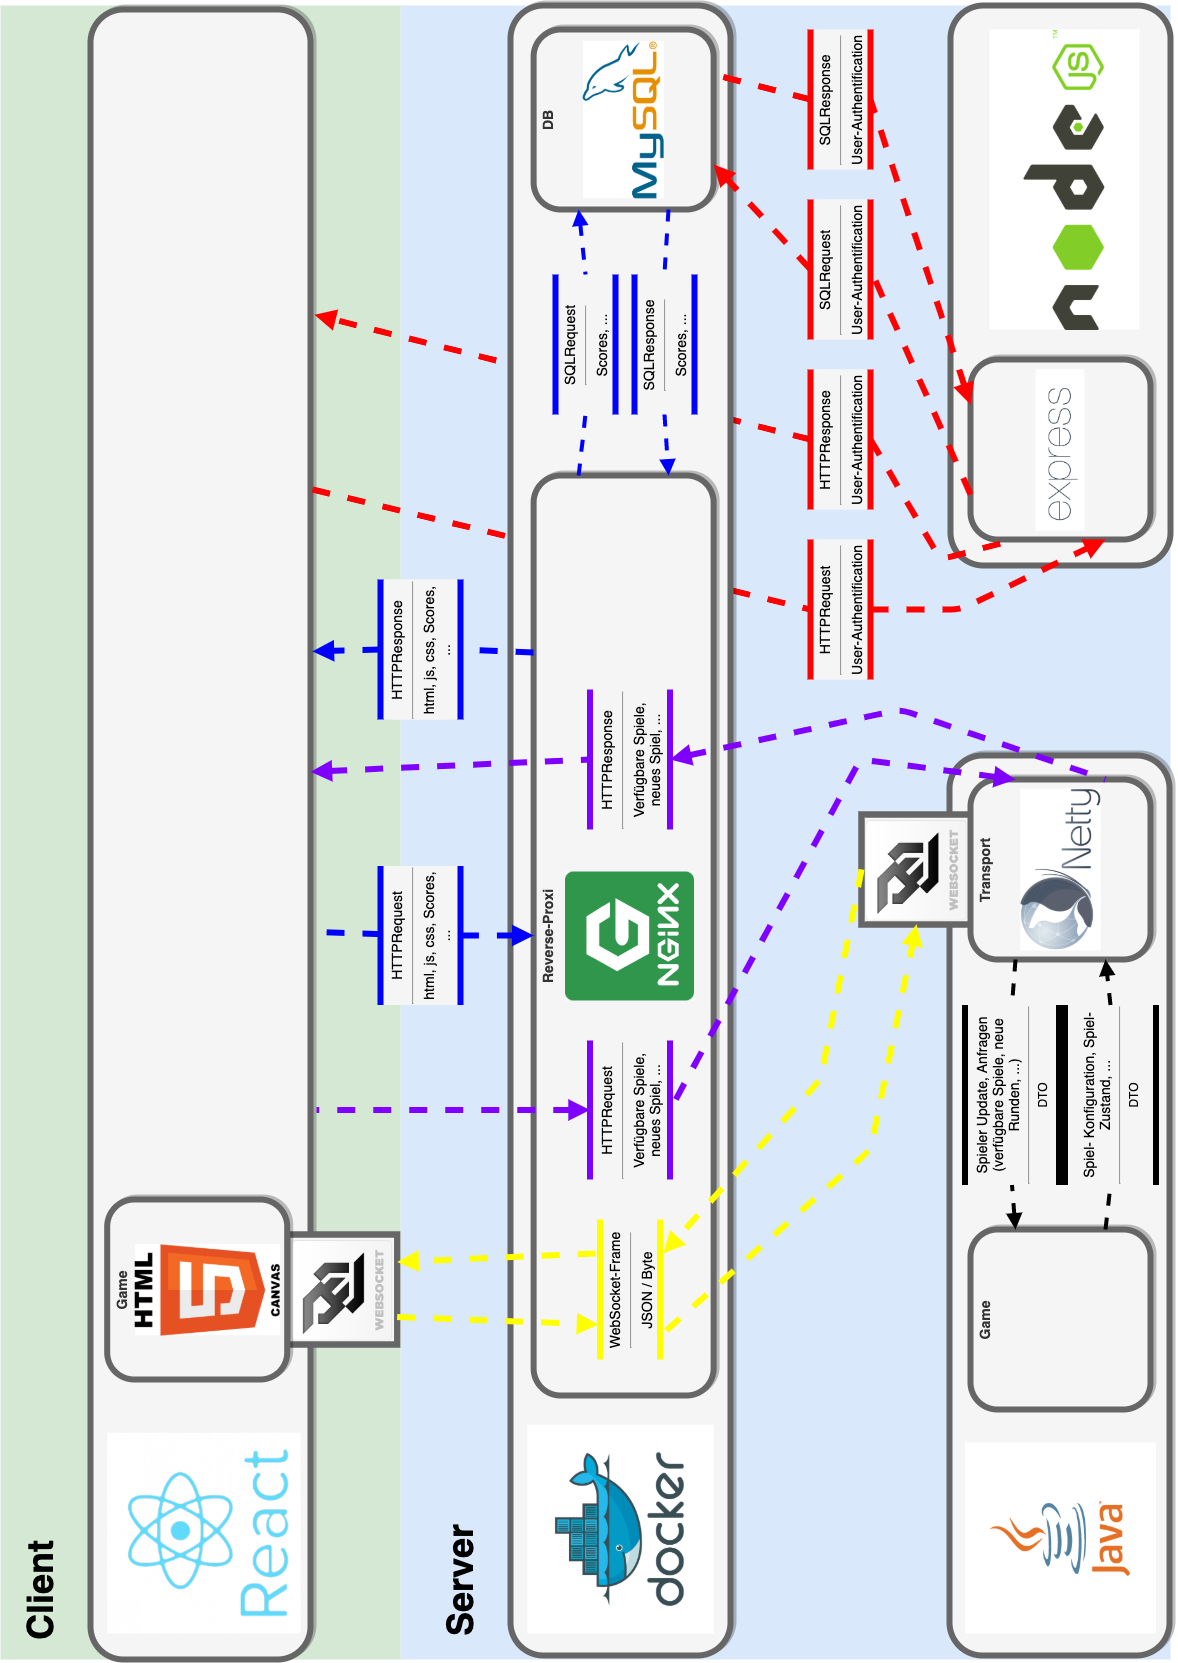
\includegraphics[scale=0.4]{figures/architecture-draft_v3.png}
            \caption{Systemarchitektur}
        \end{figure}
        \newpage

    \section{Design-Artefakte}

        \subsection{UML Moduldiagramm}
             \begin{figure}[H]
                \centering
                \makebox[\textwidth][c]{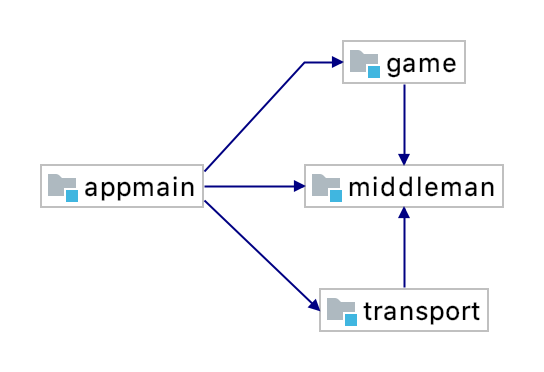
\includegraphics[width=0.5\textwidth]{figures/project modules/appmain.png}}
                \caption{UML module dependency diagram - Game Server: Module appmain}
                \label{fig:GameServerModulDiagramm}
            \end{figure}

        \subsection{UML Klassendiagramme}
            \begin{figure}[H]
                \centering
                \makebox[\textwidth][c]{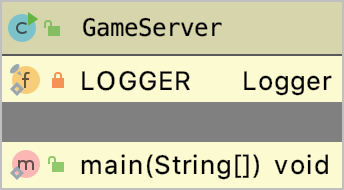
\includegraphics[width=0.5\textwidth]{figures/UML class diagrams/Package appmain light.png}}
                \caption{UML class diagrams - Game Server: Module appmain}
                \label{fig:UMLclassdiagram_Moduleappmain}
            \end{figure}
            \begin{figure}[H]
                \centering
                \makebox[\textwidth][c]{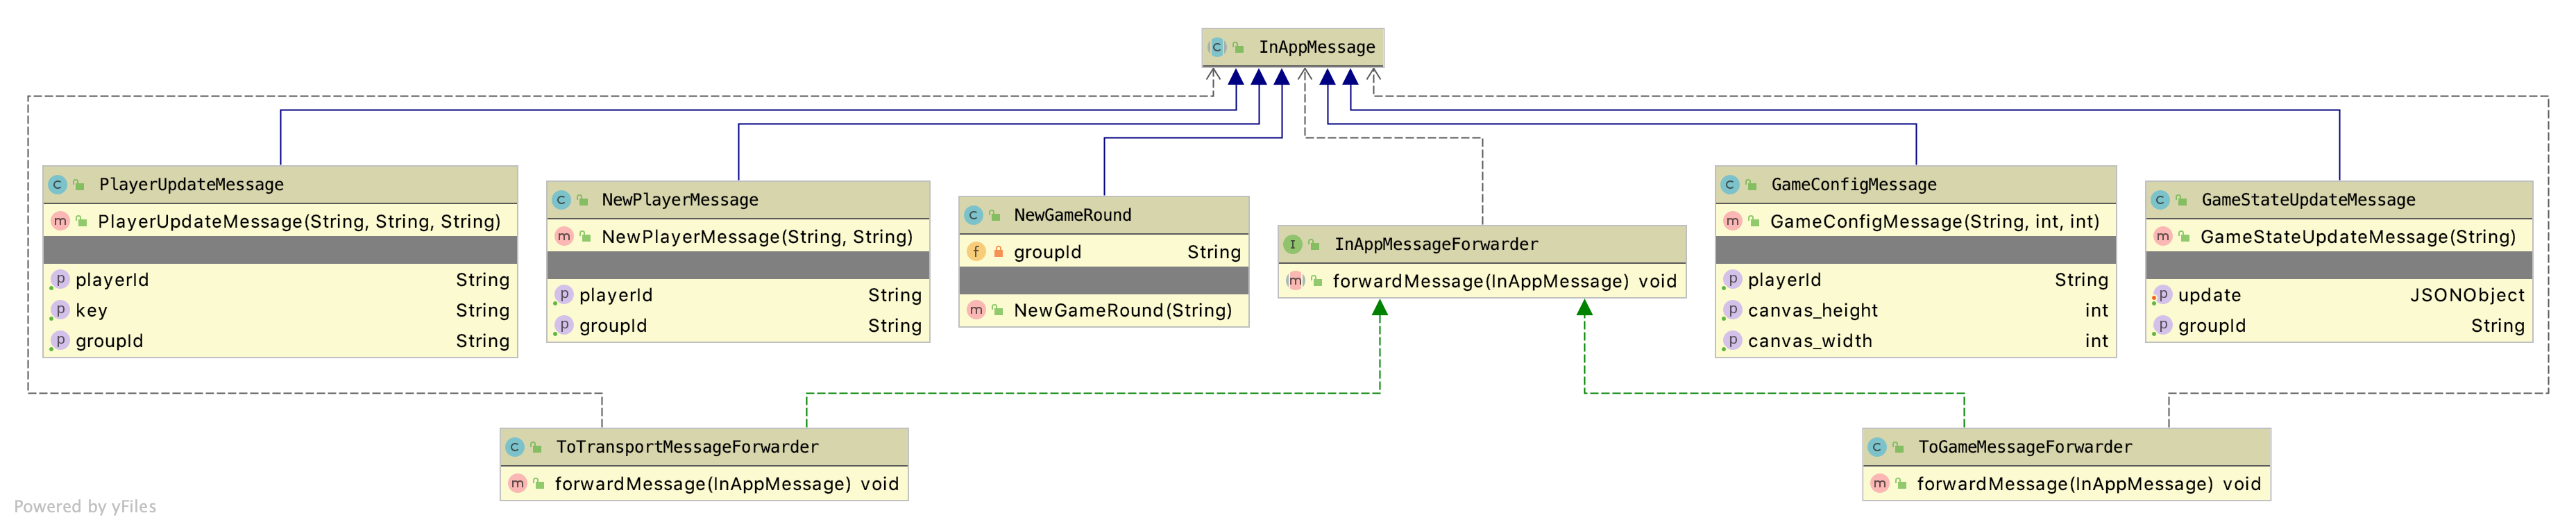
\includegraphics[width=1.1\textwidth]{figures/UML class diagrams/Package middleman light.png}}
                \caption{UML class diagrams - Game Server: Module middleman}
                \label{fig:UMLclassdiagram_Modulemiddleman}
            \end{figure}
            \newpage
            \begin{figure}[H]
                \centering
                \makebox[\textwidth][c]{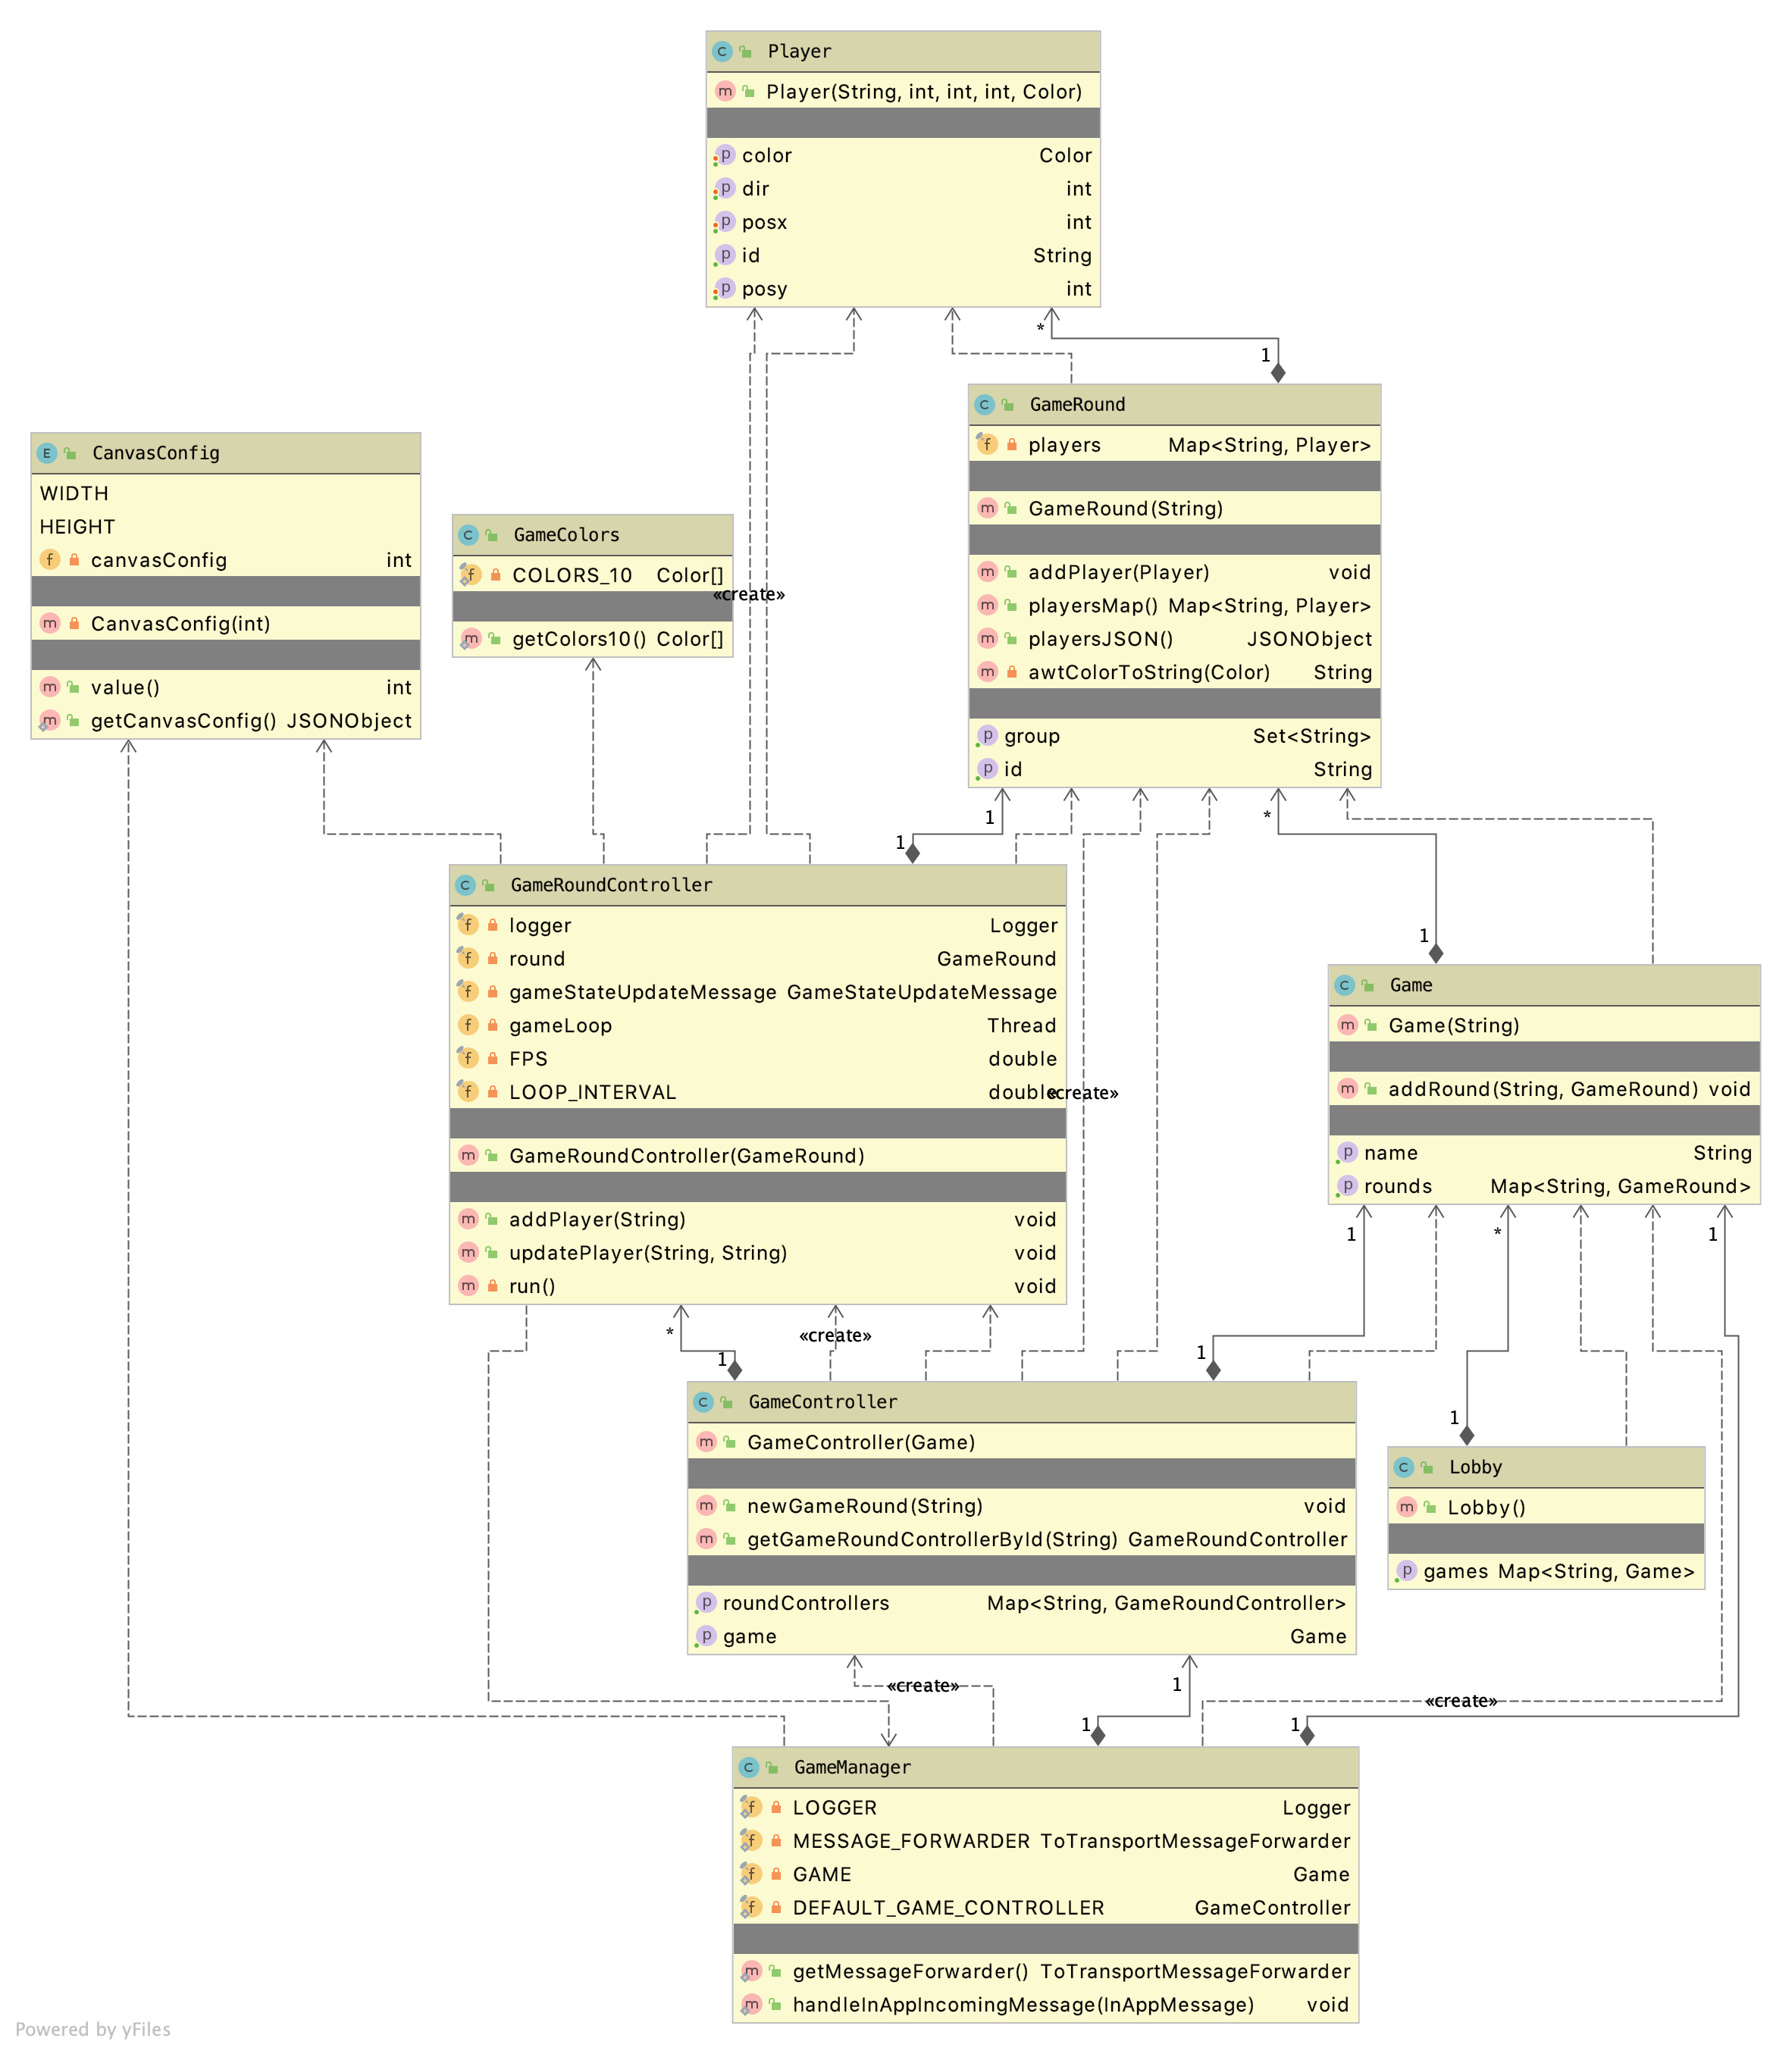
\includegraphics[width=1.1\textwidth]{figures/UML class diagrams/Package game light.png}}
                \caption{UML class diagrams - Game Server: Module game}
                \label{fig:UMLclassdiagram_Modulegame}
            \end{figure}
            \newpage
            \begin{figure}[H]
                \centering
                \makebox[\textwidth][c]{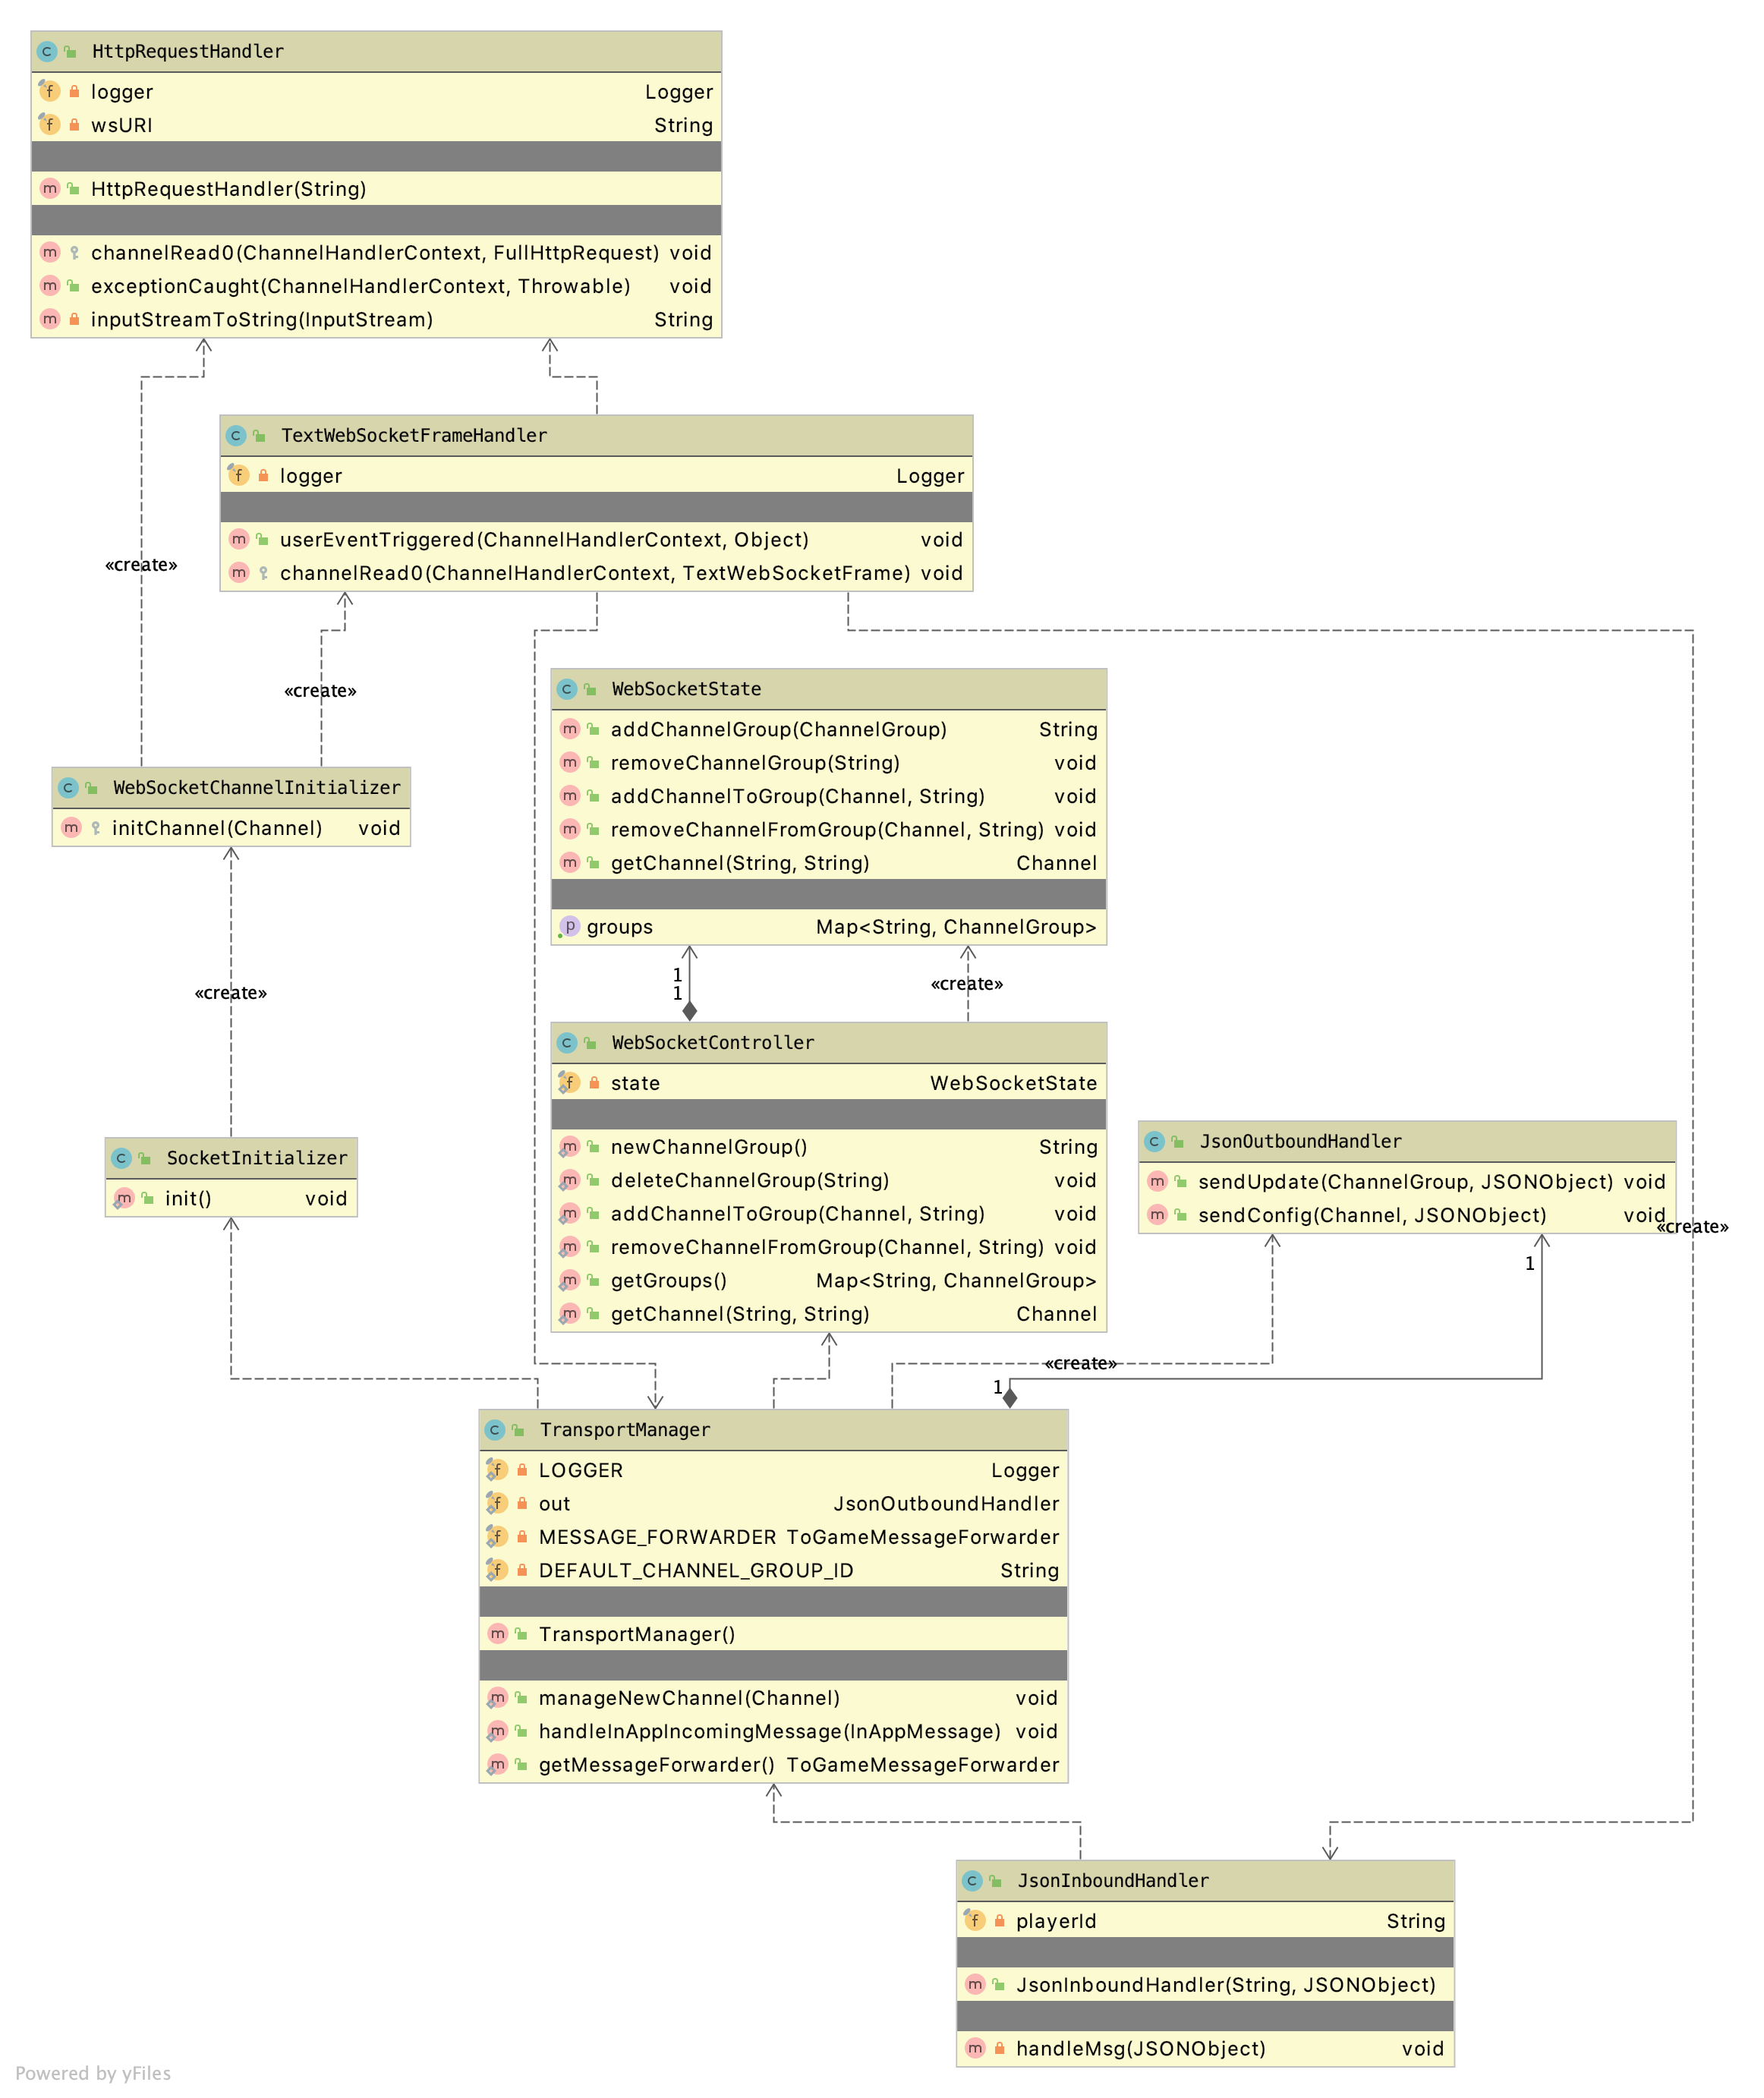
\includegraphics[width=1.1\textwidth]{figures/UML class diagrams/Package transport light.png}}
                \caption{UML class diagrams - Game Server: Module transport}
                \label{fig:UMLclassdiagram_Moduletransport}
            \end{figure}
            \newpage

    \section{Implementation}

    % TODO:
    \subsection{Game Client}
    % TODO:
    \subsection{\Gls{Game Server}}
    Wie schon in Abschnitt \ref{SoftwarearchitekturGameServer} erwähnt, wurde der \Gls{Game Server} in zwei Hauptkomponenten, die Geschläfslogik und den Transport aufgeteilt. In der Implementation entsprechen diese Komponenten den Modulen \dq ch.tron.game\dq und \dq ch.tron.transport\dq. Durch die Verwendung von Java 9 Modulen wird eine lose Kopplung gewährleistet. Wie in der Abbildung \ref{fig:GameServerModulDiagramm} zu sehen ist, existieren zwei weitere Module, \dq ch.tron.appmain\dq und \dq ch.tron.middleman\dq. Appmain dient lediglich als Einstiegspunkt für die \Gls{Game Server}-App. Das Modul Middleman wird benötigt, um die Kommunikation zwischen den Modulen Game und Transport zu ermöglichen. Es definiert eine abstrakte Klasse namens InAppMessage und einen Interface namens InAppMessageForwarder. Mit Hilfe von Subklassen von InAppMessage und den Implementationen des InAppMessageForwarders können nun Informationen, wie die Entstehung einer neuen Client-Server-Verbindung oder ein Spielupdate zwischen den Hauptkomponenten ausgetauscht werden.

    % TODO:
    \subsection{Datenbank}
    \begin{figure}[H]
    	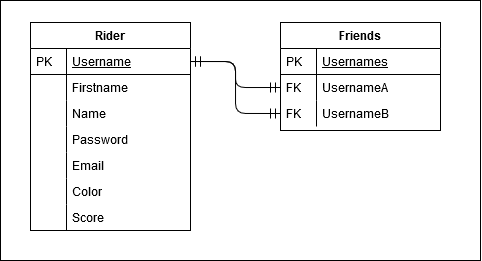
\includegraphics[scale=0.7]{figures/erm.png}
    	\caption{Datenbank - Tron Licht-Motorräder Computerspiel}
    \end{figure}
	Die Datenbank läuft auf MySQL 8.0 und wird in einem Docker-Container realisiert. In der Datenbank befinden sich die registrierten Accounts der Anwender. Zusätzlich werden auch die Freundschaftsbeziehungen zwischen den Spielern gespeichert, damit kann die Anwendung auslesen, wer in welche private \Gls{Lobby} beitreten darf.

    \section{Projektmanagement}
    Der grobe Ablauf der Arbeiten wird durch die in der Projektskizze erstellten Grobplanung bestimmt. Für die bevorstehenden Iterationen wird die Grobplanung jeweils detailliert ausgearbeitet. Nachfolgend der Iterationsplan Stand M2:

    \subsection{Iterationsplan}
    \begin{table}[H]
        \caption{Iterationsplan}
        \begin{tabularx}{\textwidth}{l l l l l l l}
            \toprule
            % Nr. & Start & Ende & Meilenstein & Ziele & Aufwand Ist & Aufwand Soll \\

            % Inception &&&&&& \\

            % 1 & 19-02-20 & 04-03-20 & M1 & Vision definiert. Geschäftsmodel definiert. Anwendungsfälle definiert und Priorisierung vorgenommen. Wichtigste nicht-funktionalen Anforderungen definiert. Recherche zu Technologien angestellt. Projektskizze erstellen. & 80 & 103 \\

            % Elaboration &&&&&& \\

            % 2 & 04-03-20 & 25-03-20 & M2 & Weitere Technologie-Recherchen vornehmen. PoC Spiel spielen. Systemarchitektur definieren. Domänenmodell erstellen. Entwicklungsumgebung aufsetzen. Github Workflow und Continuous Integration einrichten. & 80 & 74

            % 3 & 25-03-20 & 08-04-20 & M2 & Implementation Systemarchitektur. Frontend Spiel spielen. Frontend Webseite Grundstruktur. Datenbank Setup und Anbindung. Gameserver Spiel spielen modularisiert und stabilisiert. & 120 & 159 \\
            
            % Construction &&&&&& \\

            % 4 & 08-04-20 & 22-04-20 & M3 & Implementation Spielregeln, Anwendungsfälle Spiel generieren, Spiel auswählen. & 100 & \\

            % 5 & 22-04-20 & 06-05-20 & M3 & & & \\

            % 6 & 06-05-20 & M3 & & & \\
            \toprule
        \end{tabularx}
        \label{tab:Iterationsplan}
    \end{table}

    \subsection{Iterations-Assessment}
    Nachfolgend die Iterations-Assessments der vergangenen Iterationen.

    \subsubsection{Iteration 1}
    \begin{table}[H]
        \caption{Iterations-Assessment: Iteration 1}
        \begin{tabularx}{\textwidth}{l l l l}
            \toprule
            Arbeitspackete & Aufwand Soll [h] & Aufwand Ist [h] & Verantwortlicher \\
            \toprule
            Ideensammlung & 2 & 4 & alle \\
            Vision Definition & 3 & 4 & Huber \\
            Definition Anwendungsfälle, Priosierung & 10 & 15 & Akca \\
            Definition Nichtfunktionale Anforderung & 5 & 5 & Iten \\
            Projektskizze & 30 & 35 & alle \\
            Recherche Technologie & 20 & 35 & alle \\
            \bottomrule
        \end{tabularx}
        \label{tab:Iterations-Assessment: Iteration 1}
    \end{table}

    \subsubsection{Iteration 2}
    \begin{table}[H]
        \caption{Iterations-Assessment: Iteration 2}
        \begin{tabularx}{\textwidth}{l l l l}
            \toprule
            Arbeitspackete & Aufwand Soll [h] & Aufwand Ist [h] & Verantwortlicher \\
            \toprule
            Sitzungen, Diskussionen & 5 & 7 & alle \\
            Recherche Technologien & 8 & 12 & alle \\
            Systemarchitektur Artifact & 3 & 4 & Holenstein \\
            Domänenmodell & 5 & 5 & Akca \\
            PoC Gameserver & 15 & 15 & Holenstein \\
            Systemarchitektur Implementation & 10 & 12 & Huber \\
            Entwicklungsumgebung & 5 & 6 & Iten \\
            Projektmanagement Github & 5 & 5 & Huber \\
            Github Actions Continuous Integration Setup & 6 & 8 & Huber \\
            \bottomrule
        \end{tabularx}
        \label{tab:Iterations-Assessment: Iteration 2}
    \end{table}

    \subsubsection{Iteration 3}
    \begin{table}[H]
        \caption{Iterations-Assessment: Iteration 3}
        \begin{tabularx}{\textwidth}{l l l l}
            \toprule
            Arbeitspackete & Aufwand Soll [h] & Aufwand Ist [h] & Verantwortlicher \\
            \toprule
            Sitzungen, Diskussionen & 6 & 6 & alle \\
            Recherche Technologien & 15 & 17 & alle \\
            Ausformilierung Anwendungsfälle & 15 & 20 & Akca, Iten, Huber \\
            Frontend Spiel spielen & 10 & 20 & Huber \\
            Frontend Mockup & 5 & 7 & Iten \\
            Frontend Webseite Implementation & 10 & 14 & Iten \\
            Game Server Stabilisierung Kernarchitektur & 15 & 20 & Holenstein \\
            Datenbank Setup, Anbindung & 10 & 10 & Akca \\
            Projektmanagement Github & 5 & 5 & Huber, Akca \\
            Lösungsarchitektur Dokument, Artifakte & 35 & 40 & alle \\
            \bottomrule
        \end{tabularx}
        \label{tab:Iterations-Assessment: Iteration 3}
    \end{table}
    % Appendix after this
     \newpage

    \section{Appendix}
    \textit{Hinweis: Glossar-Referenznummern sind Seitennummern}
    \printglossary

\end{document}

